% Figure from MATH 556 notes, section 41 (the open mapping theorem from the ball about 0: shift and shrink). Added, not from lecture.
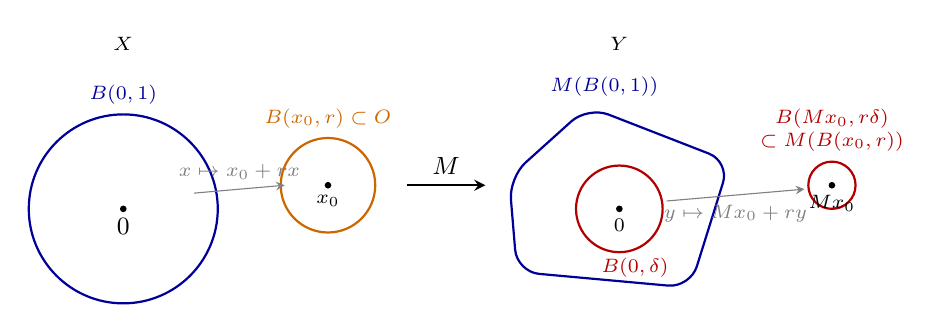
\begin{tikzpicture}[>=stealth, font=\small]
  \begin{scope}
    \node[font=\scriptsize] at (0,2.1) {$X$};
    \draw[thick, blue!60!black] (0,0) circle (1.2); \fill (0,0) circle (1.2pt) node[below] {$0$}; \node[blue!60!black, font=\scriptsize] at (0,1.45) {$B(0,1)$};
    \draw[thick, orange!80!black] (2.6,0.3) circle (0.6); \fill (2.6,0.3) circle (1.2pt) node[below, font=\scriptsize] {$x_0$}; \node[orange!80!black, font=\scriptsize] at (2.6,1.15) {$B(x_0, r) \subset O$};
    \draw[->, gray] (0.9,0.2) -- node[above, font=\scriptsize] {$x \mapsto x_0 + rx$} (2.05,0.3);
  \end{scope}
  \draw[->, thick] (3.6,0.3) -- node[above] {$M$} (4.6,0.3);
  \begin{scope}[xshift=6.3cm]
    \node[font=\scriptsize] at (0,2.1) {$Y$};
    \draw[thick, blue!60!black, rounded corners=8pt] (-1.3,-0.8) -- (0.9,-1.0) -- (1.4,0.6) -- (-0.4,1.3) -- (-1.4,0.4) -- cycle; \node[blue!60!black, font=\scriptsize, anchor=west] at (-1.0,1.55) {$M(B(0,1))$};
    \draw[thick, red!70!black] (0,0) circle (0.55); \fill (0,0) circle (1.2pt) node[below, font=\scriptsize] {$0$}; \node[red!70!black, font=\scriptsize] at (0.2,-0.75) {$B(0, \delta)$};
    \draw[thick, red!70!black] (2.7,0.3) circle (0.3); \fill (2.7,0.3) circle (1.2pt) node[below, font=\scriptsize] {$Mx_0$}; \node[red!70!black, font=\scriptsize, align=center] at (2.7,1.0) {$B(Mx_0, r\delta)$\\ $\subset M(B(x_0, r))$};
    \draw[->, gray] (0.6,0.1) -- node[below, font=\scriptsize] {$y \mapsto Mx_0 + ry$} (2.35,0.25);
  \end{scope}
\end{tikzpicture}
